\section{Description et conception des états du jeu}

\subsection{Description du jeu}

Pour jouer au RISK, il est nécessaire de disposer d'un plateau de jeu. Ce plateau est constitué : 

\begin{itemize}
    \item D'élements fixes. La carte du jeu est en effet composé des différents continents et pays du monde. 
    \item D'élements mobiles. Certains éléments sont en mouvement sur la carte. Les armées sont modifiées au gré des combats. Les cartes devront également s'afficher ou non selon les joueurs et l'avancée dans la partie.
    \newline
\end{itemize}

Tous ces éléments sur la carte du jeu, qu'ils soient fixes ou mobiles, seront caractérisés par :
\begin{itemize}
    \item Une position sur la carte. Chaque élément aura donc un attribut selon x et un attribut selon l'axe y. En effet, notre plateau de jeu sera une carte en 2 dimensions. 
    \item Un identifiant qui donnera le type de l'objet. 
\end{itemize}

\subsubsection{Les éléments fixes}

La carte est divisée en \textbf{continents}, eux-mêmes subdivisés en \textbf{pays} ou plutôt en groupe de pays puisque tous les pays du monde ne sont pas représentés sur la carte, n'ayant pas besoin d'autant d'éléments. Sur la grille composée de tuiles, un pays occupera un ensemble de tuiles proportionnellement à sa taille. Il sera frontalier d'autres pays. Dans le jeu, l'attaque ne sera alors possible qu'entre des pays frontaliers. L'esthétique choisie pour représenter les pays et les continents n'aura aucun impact sur le déroulement du jeu. Chaque continent sera représenté par une couleur principale. Chaque pays appartenant au continent héritera alors de cette couleur. 
\newline
\newline 
Les continents sont donc :
\begin{itemize}
    \item l'AFRIQUE
    \item l'ASIE
    \item l'AMERIQUE DU SUD 
    \item l'AMERIQUE DU NORD 
    \item l'EUROPE 
    \item l'OCEANIE \newline
\end{itemize}

%Les couleurs associées sont décidées avant le début de la partie : MARRON pour l'Afrique, ROUGE pour l'Asie, NOIR pour l'Amérique du Sud, JAUNE pour l'Amérique du Nord, VERT pour l'Europe et VERT FONCE pour l'Océanie. 


\subsubsection{Les éléments mobiles}

D'autres éléments ont vocation à apparaître ou disparître à l'écran. C'est notamment le cas des \textbf{armées}. 
\newline 

Au début du jeu, lorsque les territoires sont attribués à chaque joueur, le joueur déploie ses armées sur les pays qui lui sont dévolus. Sur chacun des pays occupés, un pion "armée" de la couleur du joueur viendra alors s'installer, accompagné du nombre d'armées que le joueur a décidé de positionner à cet endroit. Le nombre d'armées sur chacun des territoires est donc amené à évoluer en fonction des attaques ou défenses de chacun des joueurs. De plus, chaque joueur a la possibilité de déplacer ses armées d'un pays frontaliers à l'autre à la fin de chacun de ses tours. Enfin, les armées peuvent aussi changer de couleur si le joueur remporte un territoire. 

\vspace{0.8cm}
Les \textbf{cartes} seront également assujetties à des modifications dans leur affichage. En effet, elles ne seront affichées au joueur que si elles sont en jeu. Les cartes peuvent être dans trois états différents :
\newline 

\begin{itemize}
    \item PIOCHE : Au début du jeu, les cartes sont toutes placées dans la pioche où elles ne sont pas visibles aux joueurs.
    \item ENJEU : Lors du gain d'un territoire, le joueur pioche la première carte de la fosse. Chaque carte dispose d'une force : TANK, CANON ou SOLDAT. Ces cartes sont alors affichées.
    \item DEFAUSSE :  Quand il a entre 3 et 5 cartes, le joueur peut essayer de réaliser une combinaison qui peut lui donner un avantage en remportant des armées supplémentaires. Il défausse alors les cartes qui ne lui sont donc plus affichées. 
    Il défausse également une cartes lorsqu'il en a déjà 5 et qu'il doit piocher.
\end{itemize}

\subsection{Conception logiciel}
Le diagramme des classes pour les états est présenté sur la page suivante (figure \ref{fig:state}). Plusieurs groupes de classes commencent à se distinguer. 
Tout d'abord, un groupe de classe qui concerne uniquement \textbf{les éléments} (en orange, jaune et beige). Elles permettent de décrire le fonctionnement des éléments qui composent notre jeu. 
\newline 
\newline 
Par ailleurs, nous pouvons distinguer un groupe \textbf{conteneurs} (en vert). Celui-ci explicite tous les éléments du jeu dans un seul objet State que l'ont pourra ensuite utiliser dans le moteur du jeu.

\newpage

\begin{landscape}
    \begin{figure}[!htbp]
        \centering
        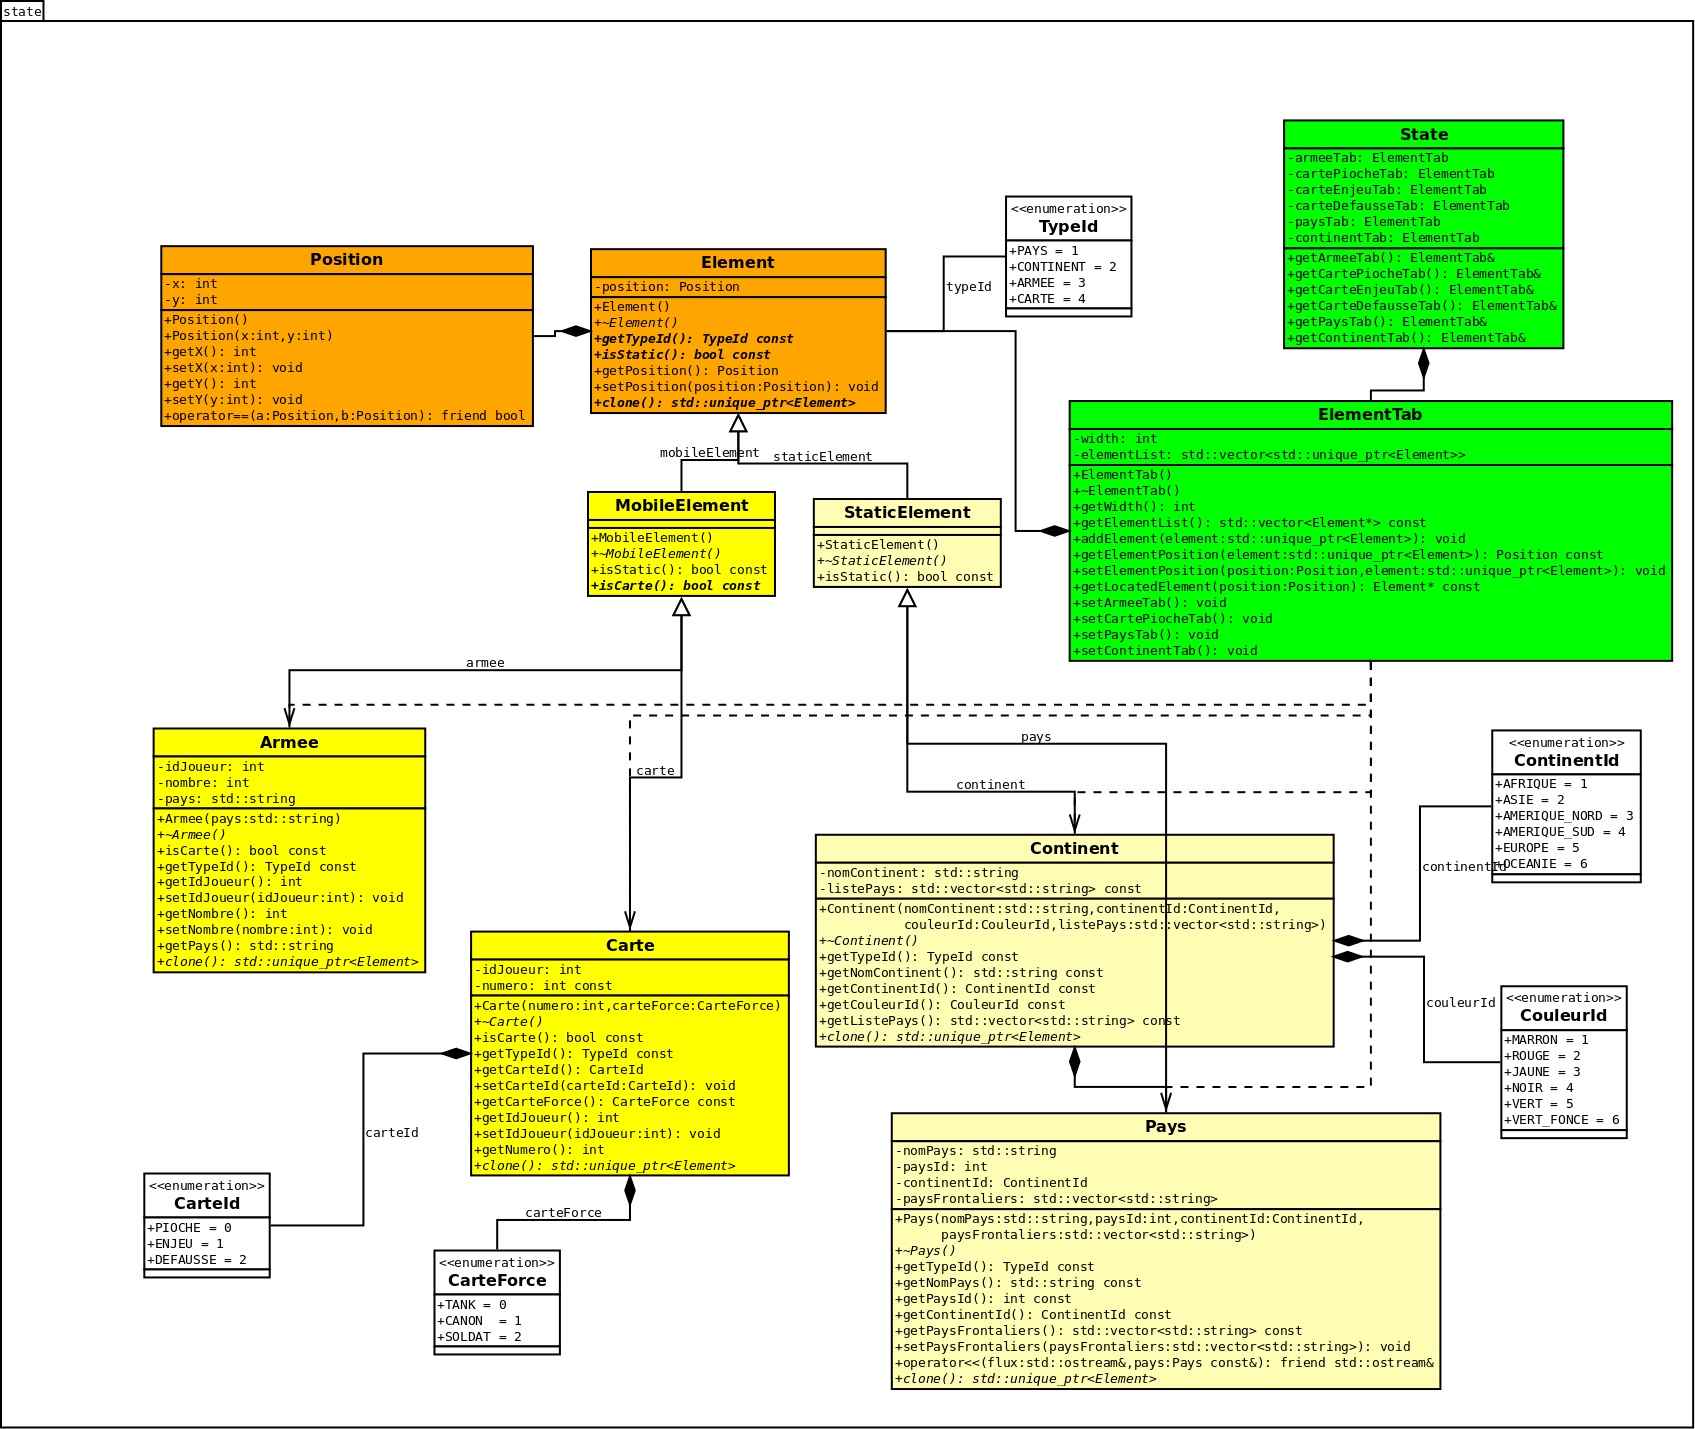
\includegraphics[width=21cm]{Images/state.png}
        \caption{Diagramme des états}
        \label{fig:state}
    \end{figure}
\end{landscape}